\documentclass[25pt, a0paper, portrait]{tikzposter}

% load packages
\usepackage{graphicx, xcolor}
\usepackage{amsmath, amssymb}
\usepackage{booktabs}
\usepackage{enumitem}

% hide package reference
\tikzposterlatexaffectionproofoff

% define poster header
\makeatletter
\renewcommand\TP@maketitle{%
   \hspace{1cm}
   \begin{minipage}{0.8\linewidth}
        \color{titlefgcolor}
        \begin{center}
          \textbf{
          \Huge{Bayesian probit models for preference classification}\\
          \vspace{1ex}
          \LARGE{An analysis of chess players' propensity for risk-taking}
          }
          \par\vspace{1em}
        \begin{tabular}{lll}
        	\Large{Lennart Oelschläger} & & \Large{Dietmar Bauer}  \\ \vspace{1ex}
        	\normalsize{lennart.oelschlaeger@uni-bielefeld.de} & & \normalsize{dietmar.bauer@uni-bielefeld.de}
    	\end{tabular}
        \end{center}
    \end{minipage}%
    \hfill
    \begin{minipage}{0.2\linewidth}
       \centering
       
\includegraphics[scale=0.25]{poster/logo.png}
    \end{minipage}
    \vspace{-3ex}
}
\makeatother

% define poster colors
\definecolor{Oeko}{HTML}{464F6E}
\colorlet{backgroundcolor}{white}
\colorlet{framecolor}{white}
\colorlet{titlefgcolor}{black}
\colorlet{titlebgcolor}{white}
\colorlet{blocktitlebgcolor}{Oeko}
\colorlet{blocktitlefgcolor}{white}
\colorlet{blocktitlebgcolor}{Oeko}
\colorlet{blockbodyfgcolor}{black}
\colorlet{innerblocktitlebgcolor}{white}
\colorlet{innerblocktitlefgcolor}{black}
\colorlet{innerblockbodybgcolor}{Oeko}
\colorlet{innerblockbodyfgcolor}{black}
\colorlet{notefgcolor}{black}
\colorlet{notebgcolor}{white}
\colorlet{notefrcolor}{Oeko}

% define block style
\defineblockstyle{mystyle}{
    titlewidthscale=0.5, bodywidthscale=1, roundedcorners=1
}{
    \draw[color=framecolor, fill=blockbodybgcolor,
    rounded corners=\blockroundedcorners] (blockbody.south west)
    rectangle (blockbody.north east);
    \ifBlockHasTitle
    \draw[color=framecolor, fill=Oeko,
    rounded corners=\blockroundedcorners] (blocktitle.south west)
    rectangle (blocktitle.north east);
    \fi
}
\useblockstyle{mystyle}

% define style changes
\renewcommand{\emph}[1]{
  \underline{\textcolor{Oeko}{\Large{\textbf{#1}}}}
}
\renewcommand{\labelitemi}{$\textcolor{Oeko}{\bullet}$}
\renewcommand{\labelenumi}{[\theenumi]}
\setitemize{labelindent=0em,labelsep=1cm,leftmargin=*}
\newcommand{\eq}[1]{
  \par\nobreak\vspace{-3ex}
  {\Large
  \begin{align}
  #1
  \end{align}
  }
  \par\nobreak\vspace{1ex}
}

% define poster content
\begin{document}

\maketitle[width=0.9\textwidth]

\begin{columns} 

\column{0.45} 

\block{Summary}{
\begin{itemize}
  \item Marketing, transportation, psychology, and other fields use probit models to analyse \emph{discrete choice behavior}. We propose a latent class model extension that allows for the \emph{classification of decider preferences} without requiring the explicit specification of the number of classes.
  \item The model is estimated in a \emph{Bayesian framework}, and the class number is determined by a \emph{Dirichlet process}. 
  \item We apply the proposed method in the context of chess, where players are classified in three classes according to their \emph{risk-taking propensity}.
\end{itemize}
}

\block{Bayesian probit models}{
Probit models are commonly rooted in the \emph{random utility framework}. They assume that deciders assign utility values to discrete choice alternatives and seek to maximize them. The utilities are modeled as a linear function of observable and unobservable factors, where the latter are assumed to follow a multivariate normal distribution. Specifically, decider $n$'s choice $y_{nt} \in \{1,\dots,J\}$ at choice occasion $t$ is explained through a matrix $X_{nt}$ of choice characteristics as
%
\eq{
\label{oelschlaeger:eq:utility}
y_{nt} = \arg \max U_{nt},\quad
U_{nt} = X_{nt} \beta + \varepsilon_{nt},\quad
\varepsilon_{nt} \sim N(0,\Sigma).
}%
We assume that \eqref{oelschlaeger:eq:utility} has been normalized for level and scale. A Bayesian analysis requires the computation of the \emph{posterior density}
%
\eq{
\label{oelschlaeger:eq:posterior}
\Pr(\beta, \Sigma \mid y, X) \propto \Pr(\beta, \Sigma) \times L(\beta, \Sigma \mid y, X).
}
%
For the prior $\Pr(\beta, \Sigma)$, it is convenient to employ independent conjugate distributions, i.e.\ the normal for $\beta$ and the inverse Wishart for $\Sigma$. The probit likelihood is the product of independent multinomial distributions
%
\eq{
\label{oelschlaeger:eq:likelihood}
L(\beta, \Sigma \mid y, X) = \prod \Pr(y_{nt} = \arg \max U_{nt}).
}
%
Evaluating \eqref{oelschlaeger:eq:likelihood} requires costly computations of the normal CDF due to the error specification in \eqref{oelschlaeger:eq:utility}. Instead, we augment $(U_{nt})_{n,t}$ as parameters [1], following truncated normals, which yields a Gibbs sampling scheme to approximate \eqref{oelschlaeger:eq:posterior}.
%
\par\vspace{2ex}
\hspace{-2ex}
\begin{minipage}{0.2\linewidth}

\includegraphics[scale = 1.2]{poster/RprobitB_sticker.png}
\end{minipage}
\begin{minipage}{0.6\linewidth}
\Large
We provide an \emph{implementation} of the Gibbs sampler in \texttt{R} via the \texttt{\{RprobitB\}} package [5].
\end{minipage}
\hspace{2ex}
\begin{minipage}{0.15\linewidth}

\includegraphics[scale = 0.6]{poster/qr_code.png}
\end{minipage}
\vspace{-3ex}
}

\block{Preference classification}{
To incorporate \emph{preference heterogeneity}, we model random variation in the coefficient vector $\beta$ across deciders using a Gaussian mixture with $C$ classes:
%
\eq{
\label{oelschlaeger:eq:mixing}
\beta_n \sim \sum s_c N(b_c, \Omega_c),
}
%
where the weights $(s_c)_c$ are Dirichlet distributed with concentration $\delta > 0$. This
%
\begin{itemize}
  \item provides an arbitrarily good approximation of the true underlying mixing distribution [4],
  \item and enables the classification of deciders with common expected preferences $b_c$ and covariances $\Omega_c$ (our focus here).
\end{itemize}
%
To avoid the need to a priori select the number $C$ of classes included, we impose a \emph{Dirichlet process prior} $DP(G, \delta)$ on the distribution \eqref{oelschlaeger:eq:mixing}, where (assuming conjugate priors for $b$ and $\Omega$) the base distribution $G$ is formed as the product of a normal and an inverse Wishart distribution [3]. The Dirichlet process integrates into the Gibbs sampler by iteratively updating $(b_c)_c$ and $(\Omega_c)_c$ using their posterior predictive distributions. The decider-specific assignments $z=(z_n)_n$ to either existing or new classes are updated via
%
\eq{
  \hspace{-2ex}
  \large
  \label{oelschlaeger:eq:dirichlet}
  \Pr(z_n = c \mid z_{-n}, \delta) = (N-1+\delta)^{-1} \cdot \begin{cases}
    |\{z_{-n} = c\}| & c = 1,\dots,C, \\
    \delta & c = C + 1,
  \end{cases}
}
%
where $z_{-n}$ denotes $z$ excluding the $n$-th element, and $N$ is the number of deciders. \par \vspace{2ex}

The \emph{impact of the concentration prior} $\delta$ on \eqref{oelschlaeger:eq:dirichlet} diminishes as $N$ increases, resulting in stable inference, as verified in our simulation: \par \vspace{2ex}
\begin{tabular}{lccccc}
\toprule[0.09 em]
           & $\delta = 0.1$ & $\delta = 0.5$ & $\delta = 1$ & $\delta = 2$ & $\delta = 10$ \\
\midrule
$N = 100$  & 1 (0.33)       & 2 (0.62)       & 2 (0.68)     & 3 (0.79)     & 4 (1.28) \\
$N = 1000$ & 3 (0.15)       & 3 (0.54)       & 3 (0.50)     & 4 (0.78)     & 5 (1.25) \\
$N = 6174$ & 3 (0.22)       & 3 (0.40)       & 3 (0.55)     & 3 (0.77)     & 4 (1.10) \\
\bottomrule[0.09 em]
\end{tabular}
}

\note[targetoffsetx=4cm, targetoffsety=-16cm, width=9cm, rotate=0, linewidth=2cm, roundedcorners=1, innersep=0.5cm]{Median $C$ for varying $N$ and $\delta$ with standard deviations. Choice data were simulated based on the estimates from the application.}

\column{0.55}

\block{Application}{
We apply the proposed model to data from an online tournament hosted on www.lichess.org [2], where $N = 6174$ participants played multiple chess games with a time limit of one minute per game. A player whos time runs out looses the game automatically. Before the start of each round, players were presented with a \emph{risky decision}: they could trade half of their clock time for the chance to earn one additional tournament point if they won the game.\par\vspace{2ex}
%
The following \emph{choice factors} potentially influence this decision: \par\vspace{1ex}
%
\begin{minipage}{0.5\linewidth}
\begin{itemize}
  \item the player's rating and the rating difference to their opponent, 
  \item whether they have the first-move advantage, 
  \item the remaining tournament time, 
  \item a winning streak (which yields extra points), 
  \item whether they opted for the risky option in the previous round, 
  \item whether they had lost in the previous round.
\end{itemize}
\end{minipage}
\hspace{2ex}
\begin{minipage}{0.5\linewidth}
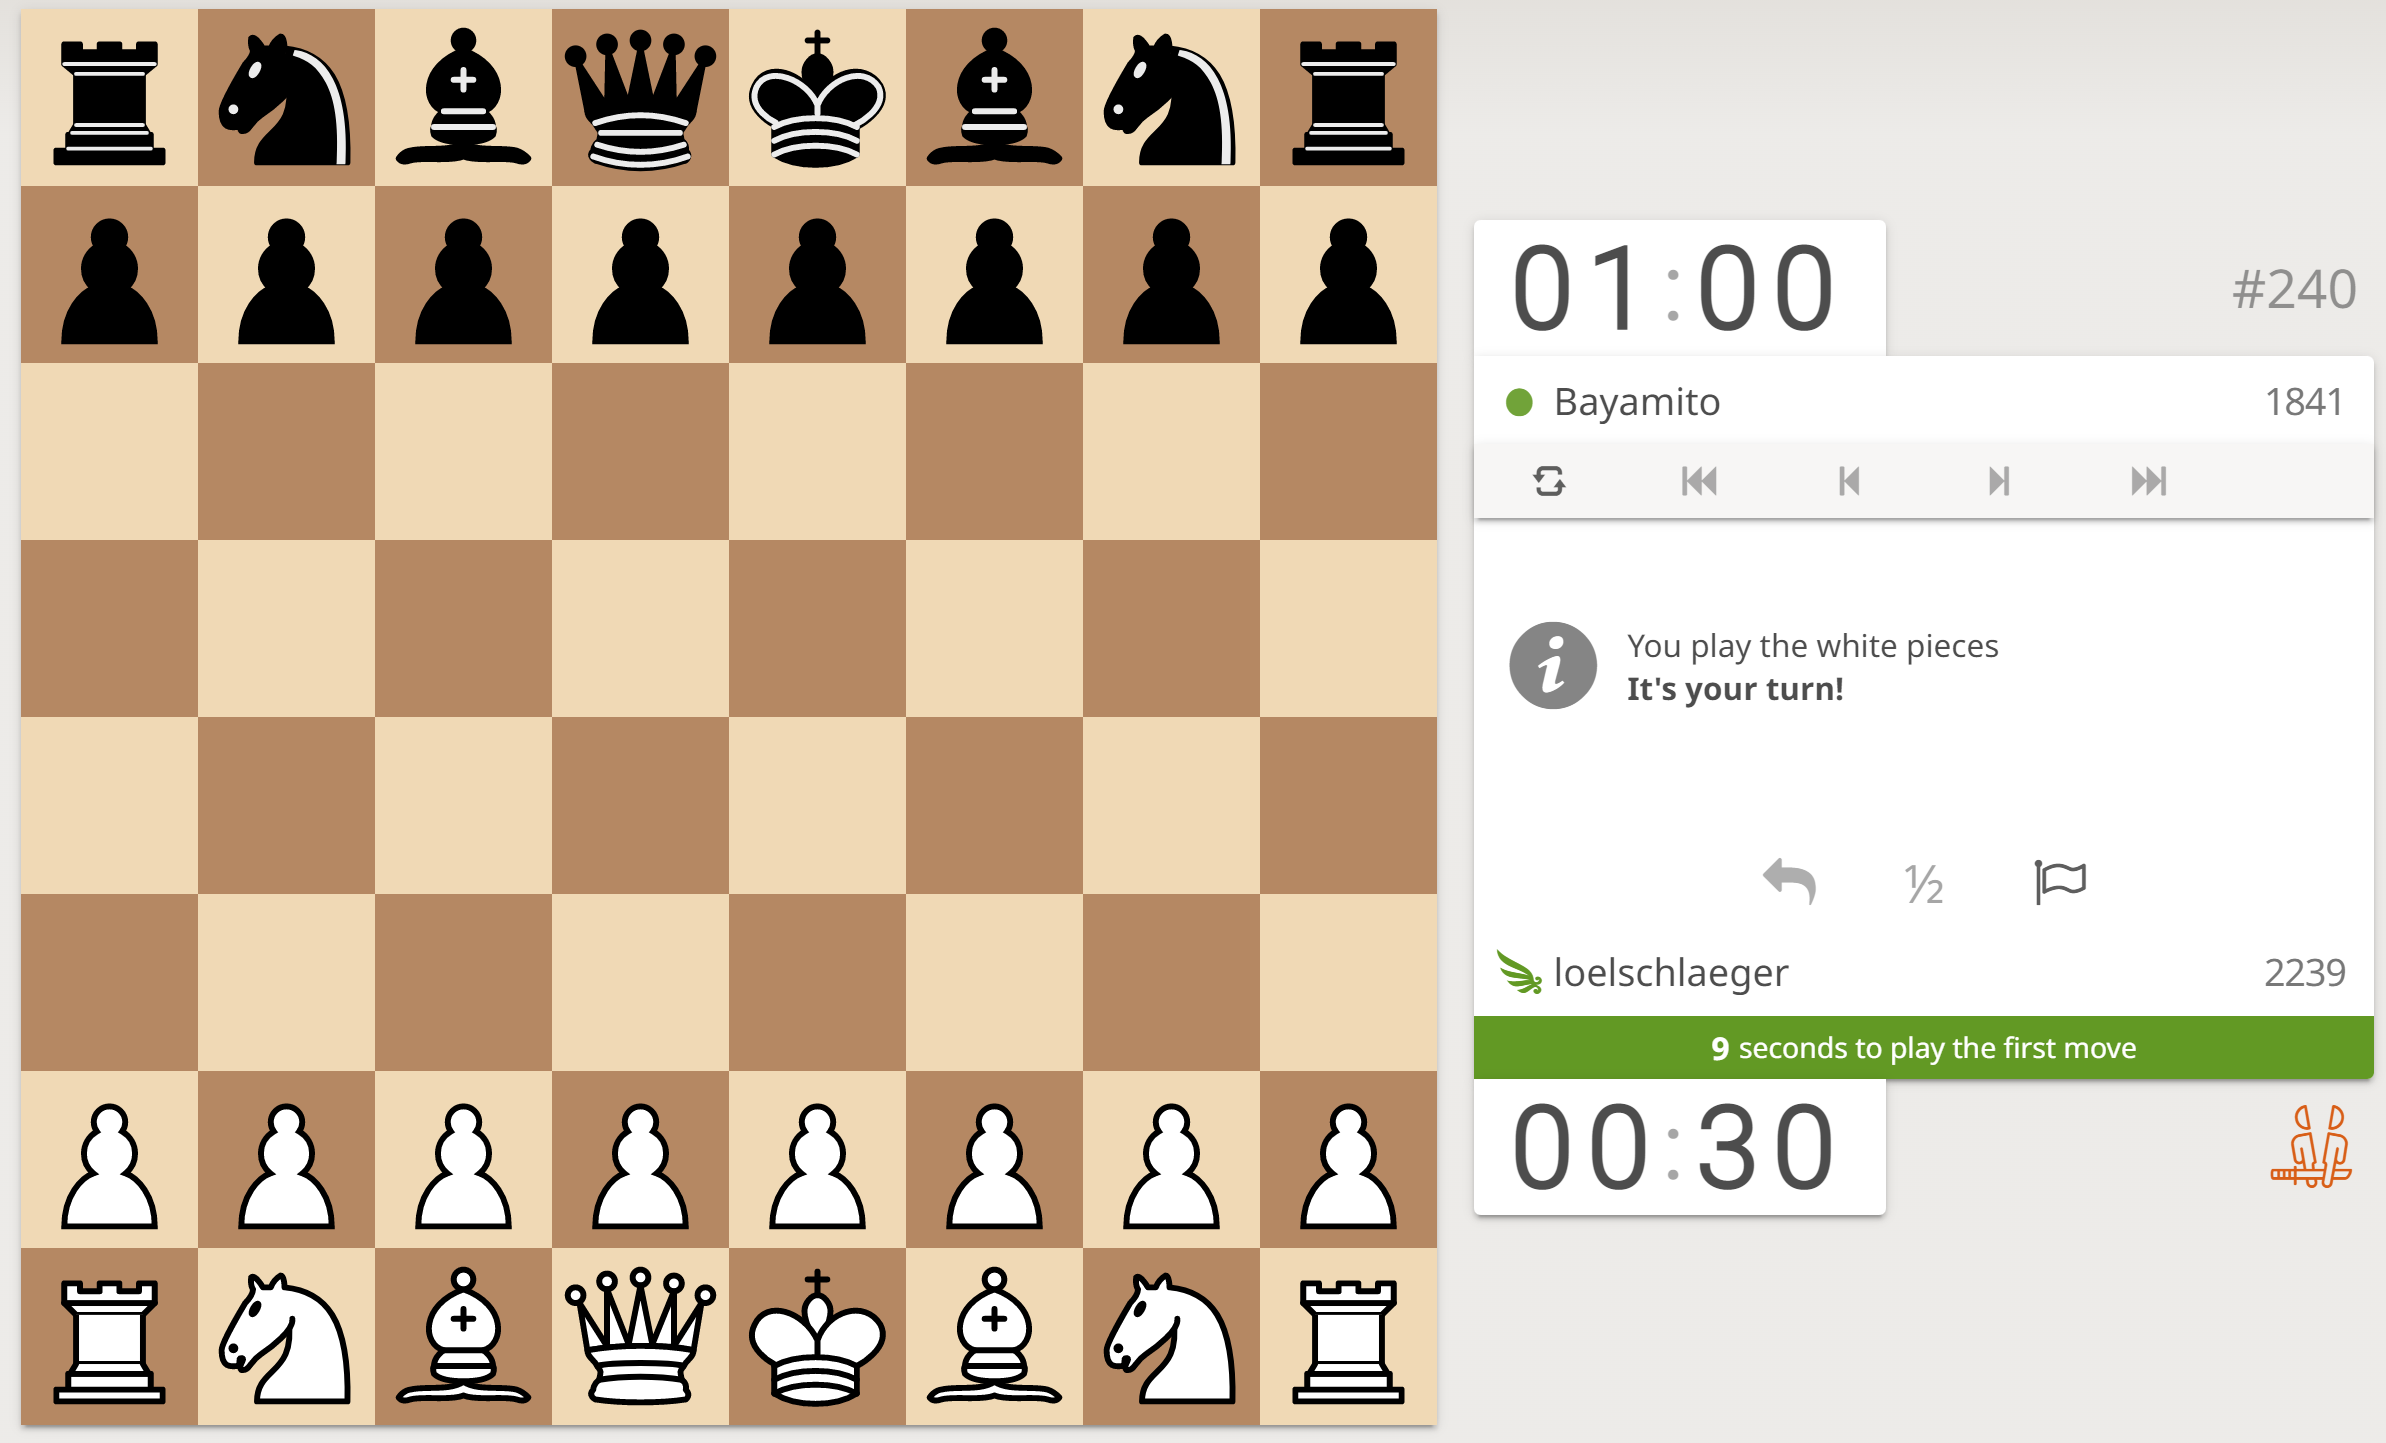
\includegraphics[scale = 0.7]{poster/lichess.png}
\end{minipage}}
%
\block{Model results}{
%
\hspace{2ex}
\begin{tabular}{lcccc}
\toprule[0.09 em]
Factor                & \multicolumn{3}{c}{Latent class probit} & Basic probit \\
\midrule
Intercept             & \multicolumn{3}{c}{-2.05 (0.03)}        & -1.94 (0.01) \\
Rating                & \multicolumn{3}{c}{-0.11 (0.01)}        & -0.08 (0.01) \\
Having first move     & \multicolumn{3}{c}{-0.04 (0.02)}        & -0.02 (0.01) \\
Minutes remaining     & \multicolumn{3}{c}{~0.04 (0.01)}        & ~0.04 (0.01) \\
On a winning streak   & \multicolumn{3}{c}{-0.27 (0.03)}        & -0.21 (0.02) \\
Took risk last round  & \multicolumn{3}{c}{~1.21 (0.02)}        & ~1.82 (0.02) \\
\midrule[0 em]
                      & Class 1        & Class 2       & Class 3       & \\
\cmidrule{2-4}
Proportion            & ~54\% (0.03)   & ~36\% (0.04)  & ~10\% (0.03)  & \\
Lost last round       & -0.98 (0.09)   & ~0.03 (0.08)  & ~1.10 (0.18)  & ~0.18 (0.01) \\
Rating difference     & ~0.10 (0.02)   & ~0.98 (0.06)  & ~1.65 (0.22)  & ~0.52 (0.01) \\
\bottomrule[0.09 em]
\end{tabular}
\par\vspace{3ex}
%
The latent class model converged to three classes that characterize different types of players:
\begin{itemize}
  \item \emph{Type 1 players} are risk-averse, rarely choosing the risky option against lower-rated opponents or after losing in the previous round.
  \item \emph{Type 2 players} decide independently of the previous game's outcome.
  \item \emph{Type 3 players} take more risks, with a higher likelihood of choosing the risky option after a loss and favoring it against weaker opponents.
\end{itemize}
\par\vspace{4ex}
%
\begin{minipage}[c]{\linewidth}
  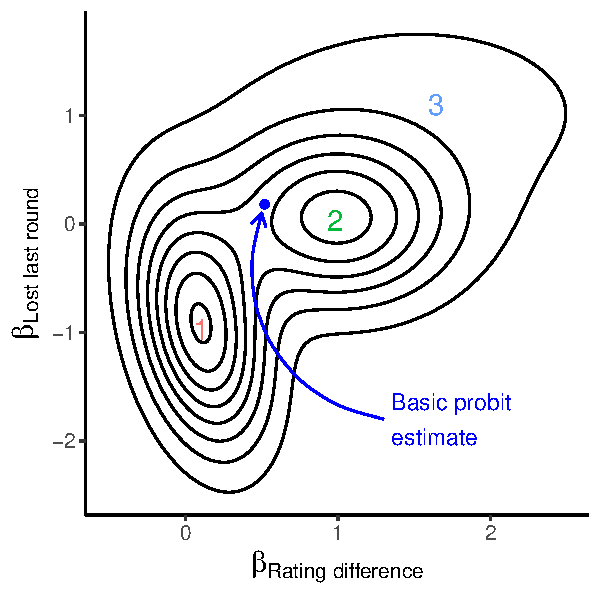
\includegraphics[width=0.5\linewidth]{poster/oelschlaeger-mixing-distr.pdf}
  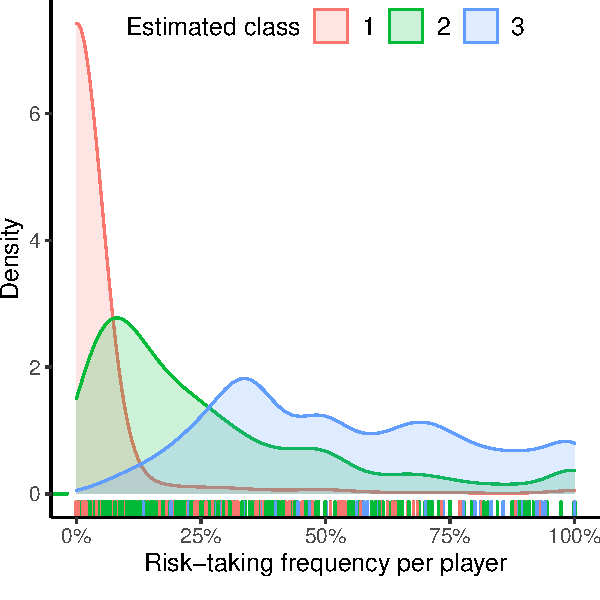
\includegraphics[width=0.5\linewidth]{poster/oelschlaeger-kd-berserk-fr.pdf}
\end{minipage}
\par\vspace{4ex}
%
Using the relative frequencies of the class allocation $z$, we can \emph{classify each player}. For example, the tournament winner is of type 2 with a probability of 78\%, while the runner-up is of type 1 with a probability of 94\%.
}

\note[targetoffsetx=8cm, targetoffsety=20.5cm, width=9.5cm, rotate=0, linewidth=2cm, roundedcorners=1, innersep=0.5cm]{Change in utility for taking the risk (ceteris paribus). Reported are the marginal posterior means with standard deviations. We fit both models using 5000 Gibbs iterations and set the concentration $\delta = 1$.}

\block{References}{
\small
\begin{enumerate}
\item {\bf Imai, K. and van Dyk, D. A.} (2005).
     A Bayesian analysis of the multinomial probit model using marginal data augmentation. \\
     {\it Journal of Econometrics}, 124.2, 311\,--\,334.
\item {\bf Lichess API} (2023).
     https://lichess.org/api/tournament/RibHfoX6.
     Data accessed on 17 February 2023.
\item {\bf Neal, R. M.} (2000).
     Markov chain sampling methods for Dirichlet process mixture models. \\
     {\it Journal of computational and graphical statistics}, 9(2), 249\,--\,265.
\item {\bf Oelschl\"ager, L. and Bauer, D.} (2021).
     Bayes Estimation of Latent Class Mixed Multinomial Probit Models.
     {\it TRB 100th Annual Meeting}.
\item {\bf Oelschl\"ager, L., Bauer, D., B\"uscher, S., and Batram, M.} (2022).
     {\it RprobitB: Bayesian Probit Choice Modeling}. \\
     R package version 1.1.2, accessible via https://CRAN.R-project.org/package=RprobitB.
\end{enumerate}
}

\end{columns}

\end{document}